\chapter{THỰC NGHIỆM} \label{chapter:ExperimentalSettings}


\section{Điều chỉnh siêu tham số} \label{sec:hyperparametersTuning}
Các siêu tham số của SAAS bao gồm các giá trị tối thiểu và tối đa cho mỗi tham số thích ứng, và các giá trị trung bình ban đầu và kích thước bước cho mỗi tham số tự thích ứng. Khác với Chagas và Wagner \cite{Chagas2021}, các siêu tham số của chúng tôi được điều chỉnh bằng thuật toán CMA-ES. Chúng tôi ngẫu nhiên chọn 21 trường hợp cho mỗi thế hệ và đánh giá các bộ siêu tham số trên chúng. Chúng tôi so sánh giá trị mục tiêu được đánh giá với giá trị mục tiêu của ACO++ trên cùng trường hợp và tính toán phần trăm cải thiện so với ACO++. Cuối cùng, chúng tôi lấy trung bình phần trăm cải thiện trên 21 trường hợp để làm fitness cho CMA-ES. Chúng tôi cập nhật quần thể bằng cách giữ lại hai cá thể tốt nhất từ hai thế hệ trước. Sau khi điều chỉnh, chúng tôi đánh giá hai cá thể tốt nhất từ hai thế hệ cuối cùng trên tất cả các trường hợp. Chúng tôi chọn cá thể tốt hơn làm bộ siêu tham số cuối cùng cho thuật toán.

Chúng tôi sử dụng các siêu tham số giống như Chagas và Wagner cho BRKGA, ACO và ACO++ \cite{Chagas2021}, ngoại trừ ILS vì nó không có siêu tham số. Các siêu tham số này đã được tìm thấy thông qua quá trình điều chỉnh. Chagas và Wagner đã gom nhóm các trường hợp có cùng định dạng \texttt{XXX\_YY\_ZZZ} để phục vụ cho quá trình điều chỉnh siêu tham số. Tổng cộng, benchmark có 48 nhóm. Đối với mỗi nhóm trường hợp và mỗi thuật toán, Chagas và Wagner đã thực hiện 5.000 thí nghiệm \cite{Chagas2021}, dẫn đến 240.000 thí nghiệm cho mỗi thuật toán. Ngược lại, chúng tôi điều chỉnh SAAS 
chỉ với 45.000 thí nghiệm. Lưu ý rằng một thí nghiệm tương đương với việc thực thi thuật toán cho một trường hợp trong benchmark.

% Viết thêm


\section{Bộ benchmark được sử dụng} \label{sec:problem}
ThOP benchmark \cite{8477853} bao gồm 432 trường hợp, mỗi trường hợp có các đặc điểm riêng biệt về số lượng thành phố, số lượng vật phẩm, kích thước ba lô, thời gian di chuyển tối đa và sự tương quan giữa trọng lượng và lợi nhuận của các vật phẩm. Các trường hợp này được lấy từ TTP benchmark \cite{10.1145/2576768.2598249} bằng cách loại bỏ các vật phẩm liên quan đến các thành phố bắt đầu và kết thúc và thêm thời gian di chuyển tối đa. Các đặc điểm của các trường hợp:

\begin{itemize}
    \item Số lượng thành phố: 51, 107, 280 hoặc 1000 (từ các trường hợp TSP: \textit{eil51}, \textit{pr107}, \textit{a280}, \textit{dsj1000}).
    \item Số lượng vật phẩm trên mỗi thành phố: \textit{01}, \textit{03}, \textit{05} hoặc \textit{10}.
    \item Sự tương quan giữa trọng lượng và lợi nhuận: Không tương quan (uncorrelated, \textit{unc}), không tương quan với trọng lượng tương tự (uncorrelated with similar weights, \textit{usw}) hoặc bị giới hạn và tương quan mạnh (bounded and strongly correlated, \textit{bsc}).
    \item Kích thước ba lô: Kích thước ba lô có thể là \textit{01}, \textit{05} hoặc \textit{10} lần kích thước ba lô nhỏ nhất.
    \item Thời gian di chuyển tối đa: Được xác định bởi các lớp \textit{01}, \textit{02} hoặc \textit{03}, tương ứng với 50\%, 75\% và 100\% thời gian tham chiếu cho mỗi trường hợp trong bài báo gốc của ThOP \cite{8477853}.
\end{itemize}

Mỗi trường hợp được biểu thị ở định dạng \texttt{XXX\_YY\_ZZZ\_WW\_TT}, trong đó \texttt{XXX} biểu thị loại trường hợp TSP, \texttt{YY} biểu thị số lượng vật phẩm trên mỗi thành phố, \texttt{ZZZ} biểu thị loại ba lô, \texttt{WW} biểu thị kích thước ba lô và \texttt{TT} biểu thị thời gian di chuyển tối đa. Ví dụ: \texttt{pr107\_05\_bsc\_01\_01} biểu thị: trường hợp có 107 thành phố pr107 của TSP benchmark; 5 vật phẩm trên mỗi thành phố có trọng lượng và lợi nhuận phụ thuộc lẫn nhau, bị giới hạn; kích thước ba lô và giới hạn thời gian nhỏ nhất như đã nêu.

\section{Thiết lập thực nghiệm} \label{sec:experimentsSetup}

Chúng tôi so sánh chất lượng của các giải pháp thu được bởi phương pháp đề xuất của chúng tôi SAAS và bởi các phương pháp trước đây. Các phương pháp trước đây được dùng trong thực nghiệm bao gồm ILS~\cite{8477853}, BRKGA~\cite{8477853}, ACO~\cite{CHAGAS2020708}, và ACO++~\cite{Chagas2021} nhưng không bao gồm GA~\cite{9185848} do chúng tôi không thể tiếp cận mã nguồn của nó. Để có sự so sánh công bằng, chúng tôi đã chạy thực nghiệm cho tất cả các phương pháp trên cùng một máy tính với Intel(R) Core(TM) i7-8750H @ 2.20GHz.

Vì tất cả các thuật toán đều có yếu tố ngẫu nhiên, chúng tôi thực hiện 30 lần chạy độc lập trên mỗi trường hợp trong benchmark. Đối với SAAS, chúng tôi sử dụng bộ tham số tốt nhất được tìm thấy bởi quá trình điều chỉnh của chúng tôi cho tất cả các trường hợp trong ThOP benchmark. Đối với BRKGA, ACO và ACO++, chúng tôi sử dụng các bộ siêu tham số tốt nhất tương ứng với các nhóm trường hợp được tìm thấy trong bài báo ACO++ \cite{Chagas2021}. Xin lưu ý rằng chúng tôi giới hạn thời gian thực thi của mỗi trường hợp trong ThOP benchmark là $\left \lceil 0.1m \right \rceil$ giây với $m$ là số lượng vật phẩm trong trường hợp tương ứng \cite{8477853}.

Bên cạnh so sánh giá trị mục tiêu của lời giải, chúng tôi có tiến hành kiểm định Wilcoxon signed-rank cho 2 phương pháp tốt nhất để kiểm tra độ tin cậy của so sánh. 

% Viết thêm

\section{Kết quả thực nghiệm}
\label{sec:result}
\subsection{Kết quả thực nghiệm so sánh lời giải của các thuật toán}
\label{sec:solutionApproaches}

Đầu tiên chúng tôi tiến hành thực nghiệm so sánh kết quả lời giải của các thuật toán bằng cách so sánh tỉ lệ giá trị mục tiêu ở mỗi trường hợp với lời giải tốt nhất được tìm thấy. Ở mỗi thuật toán, chúng tôi tính giá trị tỉ lệ này bằng việc tính trung bình giá trị mục tiêu của 30 lần chạy độc lập cho một trường hợp. Sau đó tính tỉ lệ so với giá trị mục tiêu của lời giải tốt nhất được tìm thấy cho trường hợp đó qua thực nghiệm của chúng tôi. Giá trị tỉ lệ này càng cao thì hiệu suất của thuật toán hiện tại càng tốt trong trường hợp đó. Kết quả của thực nghiệm này được thể hiện qua Hình \ref{fig:profit_ratio}.

Qua kết quả thực nghiệm cho thấy được rằng ILS và BRKGA thể hiện hiệu suất thấp hơn hẳn so với 3 thuật toán dựa trên giải thuật tối ưu hóa đàn kiến ACO, ACO++, SAAS với 2 biểu đồ nhiệt có bảng màu nhạt hơn. Ta có thể thấy rằng ILS và BRKGA thể hiện tốt với cái trường hợp có kích thước nhỏ ở số lượng thành phố hoặc số lượng vật phẩm ở mối thành phố. Điều này thể hiện qua biểu đồ nhiệt của 2 thuật toán này đậm hơn ở 2 viền: viền trái và viền dưới của biểu đồ.

Các thuật toán dựa trên giải thuật đàn kiến (ACO, ACO++, SAAS) thể hiện hiệu suất ổn định trên toàn bộ thang đo với các biểu đồ nhiệt có bảng màu đậm ở hầu hết các trường hợp. ACO++ và SAAS là 2 thuật có biểu đồ nhiệt đậm nhất trong 5 thuật toán chúng tôi đã thử nghiệm. ACO++ thể hiện rất tốt với biểu đồ nhiệt đậm và có nhiều ký hiệu hình thoi (tìm ra được nhiều lời giải tốt nhất), tuy nhiên thuật toán SAAS của chúng tôi có biểu đồ nhiều đậm hơn và dày đặc các ký hiệu hình thoi hơn (tìm ra được nhiều lời giải tốt nhất hơn). SAAS thành công tìm ra được lời giải tốt nhất cho 330 trường hợp trên 432 trường hợp của benchmark trong khi đó ACO++ chỉ tìm được lời giải tốt nhất trên 180 trường hợp.

Với biểu đồ nhiệt của thuật toán SAAS của chúng tôi, ta có thể thấy các ký hiệu hình thoi dày đặt ở phía bên trái biểu đồ và thưa dần về bên phải bắt đầu từ các trường hợp có tiền tố  \texttt{a280\_01} trở đi. Điều này xảy ra là bởi vì thuật toán của chúng tôi không có đủ thời gian để tìm ra lời giải tốt nhất. Các trường hợp ở bên phải các trường hợp có tiền tố  \texttt{a280\_01} là các trường hợp của số lượng thành phố lớn (280 và 1000 thành phố) nên để tìm được lời giải tốt thuật toán của chúng tôi cần nhiều thời gian hơn bởi vì việc tìm kiếm các giá trị tham số thực thi trong quá trình chạy. 

\begin{figure}
    \centering
    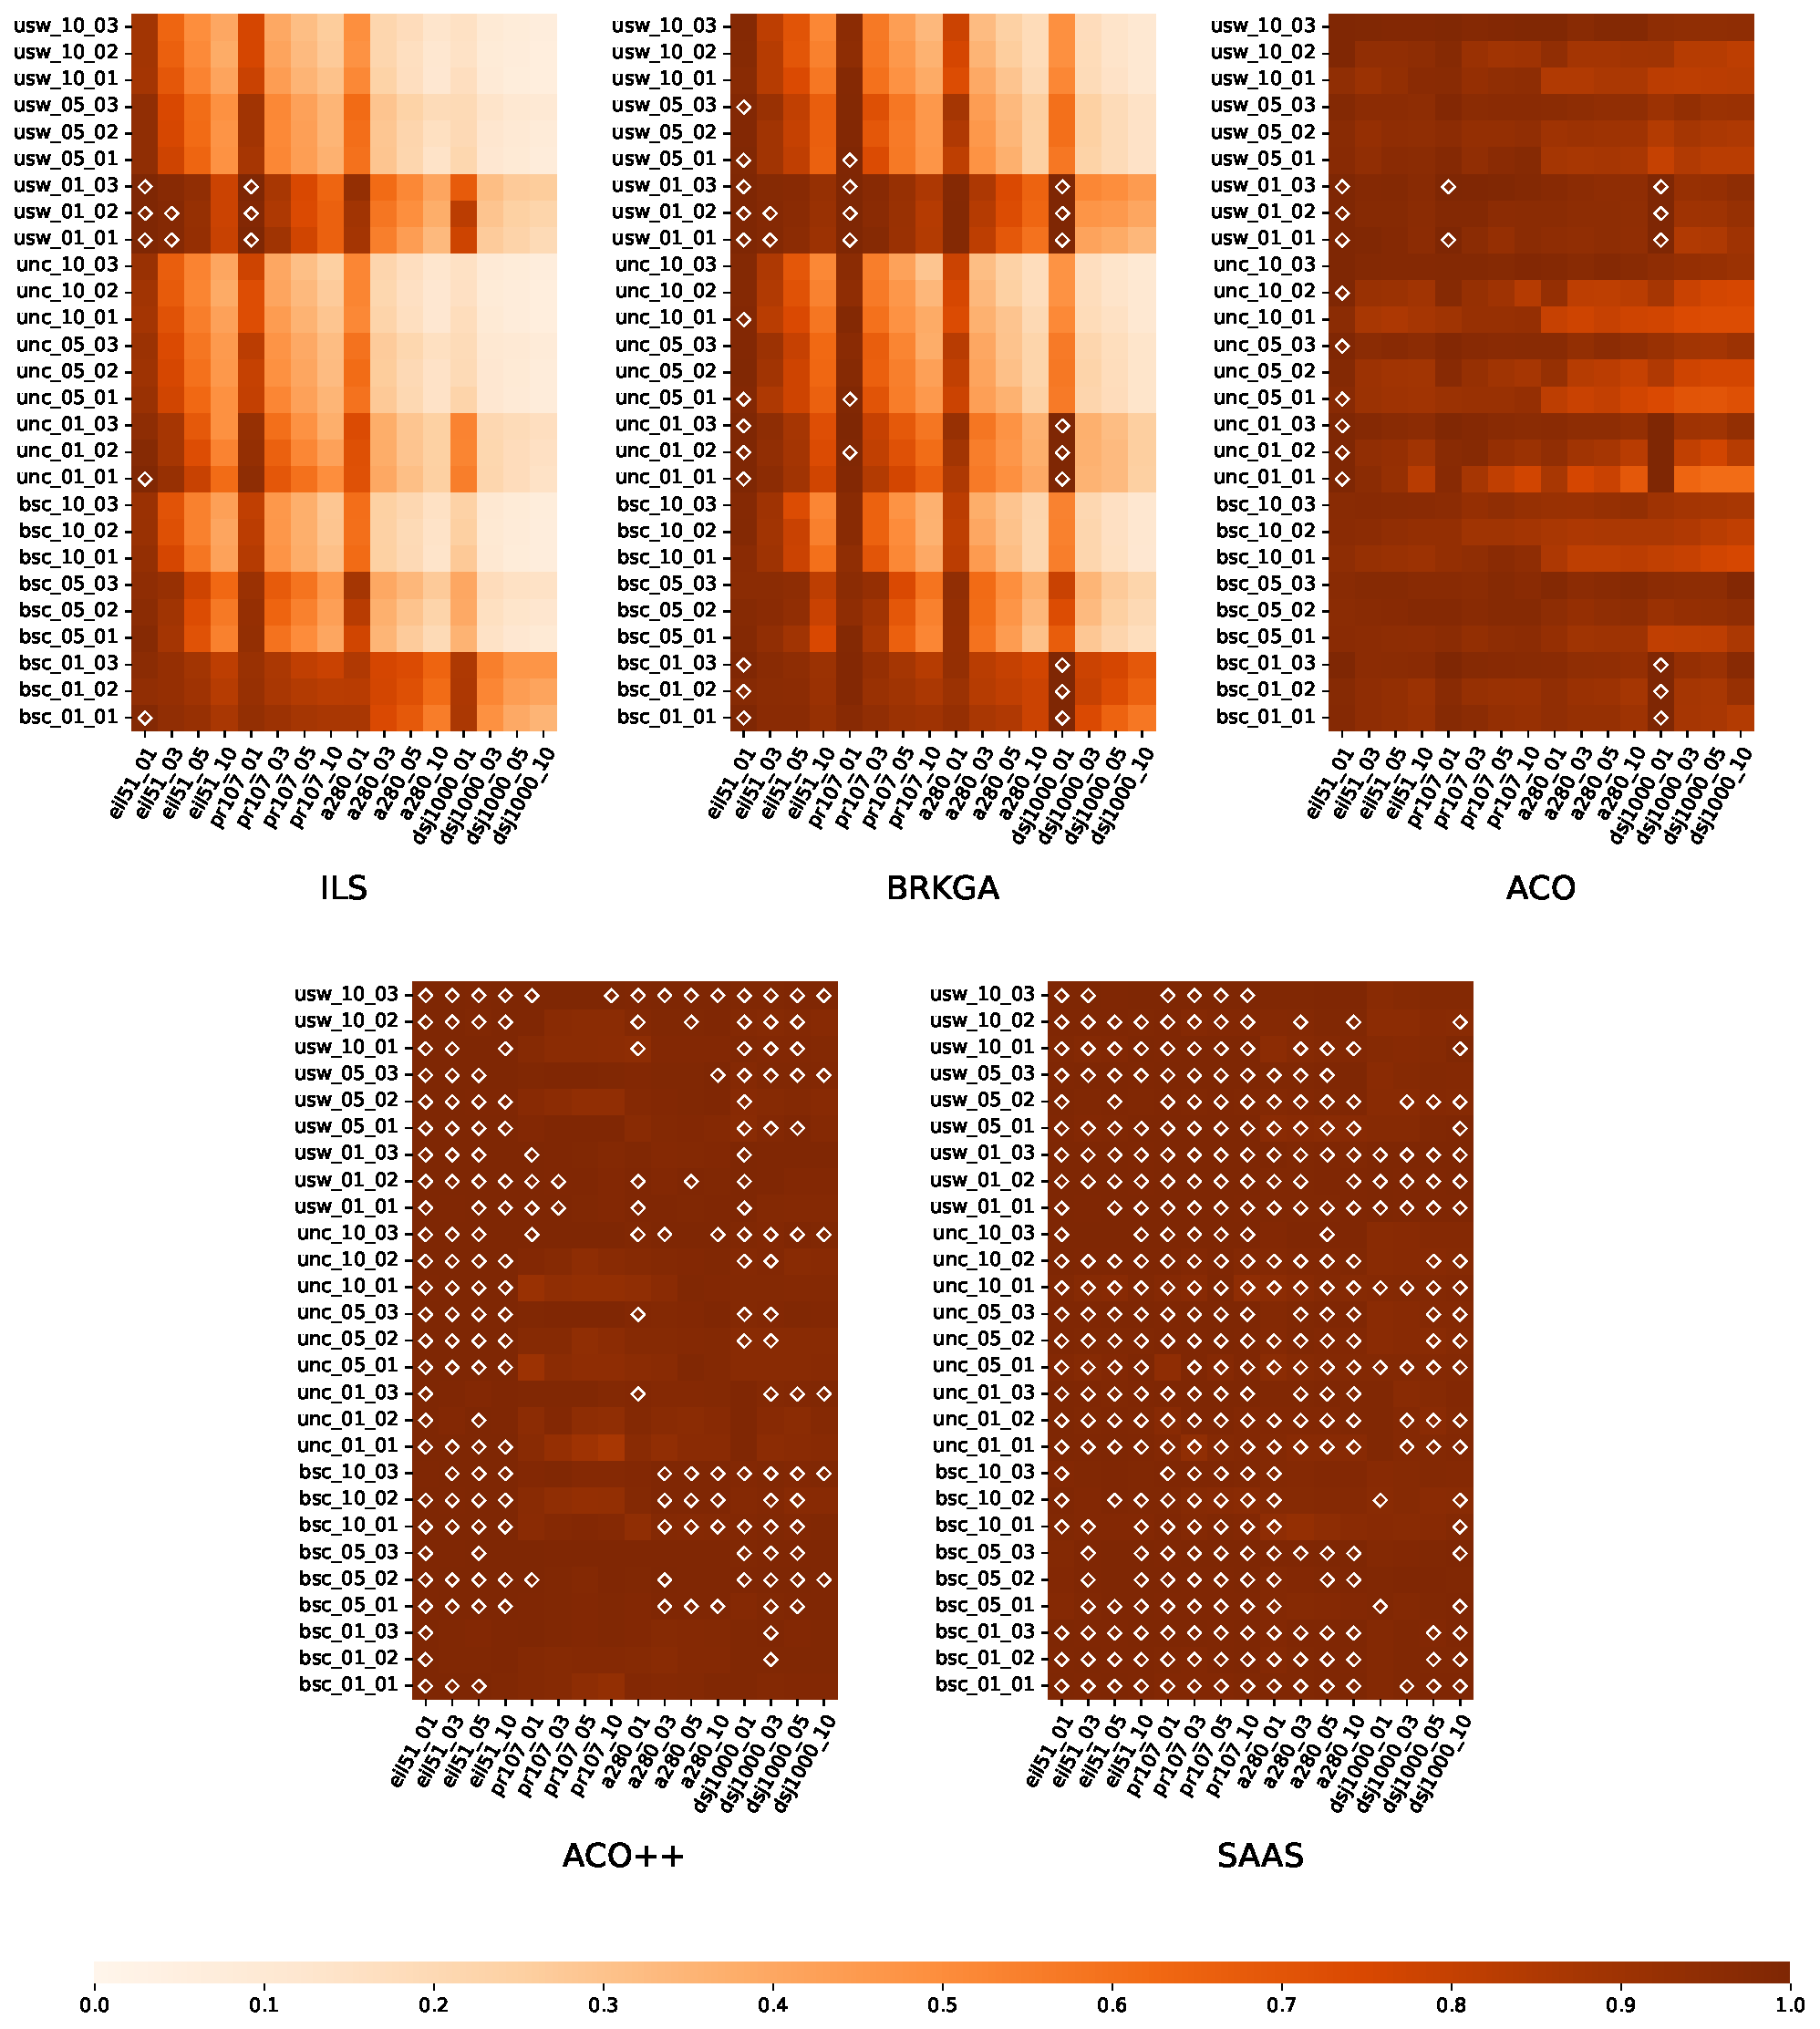
\includegraphics[width=\textwidth]{Figures/profit_ratio.pdf}
    \caption[Kết quả thực nghiệm so sánh lời giải của các thuật toán.]{Biểu đồ nhiệt của mỗi thuật toán thể hiện tỉ lệ kết quả lời giải trên từng trường hợp của thuật toán đó, với lời giải tốt nhất được tìm thấy cho trường hợp đó trong tất cả thực nghiệm. Mỗi ô trên mỗi biểu đồ nhiệt thể hiện một trường hợp. Độ đậm nhạt ở mỗi ô thể hiện tỉ lệ lời giải, màu sắc càng đậm thể hiện lời giải có kết quả gần bằng với lời giải tốt nhất được tìm thất. Ký hiệu hình thoi ở một số ô thể hiện thuật toán đó tìm ra lời giải tốt nhất được tìm thấy cho trường hợp tại vị trí đó.}
    \label{fig:profit_ratio}
\end{figure}
\subsection{Kết quả thực nghiệm so sánh hiệu suất giữa các thuật toán}
\label{sec:winpercent}
Để so sánh các cặp thuật toán với nhau về mặt số lượng lời giải tốt, chúng tôi đã xây dựng bảng \ref{tab:winpercent}, bảng thống kê phần trăm các lời giải của mỗi thuật toán tìm ra lời giải có chất lượng tốt hơn hoặc ngang bằng so với thuật toán khác. Ở mỗi cặp thuật toán, chúng tôi tính giá trị phần trăm số lượng dựa trên lời giải tốt nhất ở hai thuật toán của 30 lần chạy độc lập ở mỗi trường hợp. 

\begin{table}[ht!]
  \begin{center}      
        \begin{tabular}{lrrrrr}
        \toprule
        i $\downarrow$ \ \ \ \ j $\rightarrow$  & ILS & BRKGA & ACO & ACO++ & SAAS \\
        \midrule
        ILS & - & 2.55\% & 4.40\% & 2.55\% & 2.31\% \\
        BRKGA & 100.00\% & - & 16.20\% & 8.80\% & 7.18\% \\
        ACO & 97.22\% & 87.27\% & - & 5.79\% & 4.86\% \\
        ACO++ & 99.54\% & 95.83\% & 97.69\% & - & 41.90\% \\
        SAAS & 99.77\% & 97.92\% & 98.61\% & 78.24\% & - \\
        \bottomrule
        \end{tabular}
      \caption[Kết quả thực nghiệm so sánh hiệu suất giữa các thuật toán.]{
      \label{tab:winpercent}Bảng thống kê phần trăm chất lượng các lời giải của thuật toán i tốt hơn hoặc ngang bằng so với lời giải của thuật toán j.}
  \end{center}
\end{table}

Kết quả được thể hiện trong bảng này chứng thực cho những gì thể hiện trên hình \ref{fig:profit_ratio}. BRKGA hoàn toàn áp đảo ILS với tỉ lệ là 100\% và các thuật toán dựa trên thuật toán đàn kiến thể hiện hiệu suất tốt hơn với hai thuật ILS và BRKGA. Thuật toán của chúng tôi SAAS và ACO++ đều thiện hiện hiệu suất vượt trội so với các thuật toán khác với hơn 95\% số lượng các trường hợp trên benchmark. SAAS có số lượng lời giải tốt hơn 78.24\% ACO++. 
\subsection {So sánh thống kê Wilcoxon signed-rank}
Với hiệu suất tương đối và dẫn đầu của cả hai thuật toán SAAS và ACO++, chúng tôi tiến hành thử nghiệm Wilcoxon signed-rank để xác minh sự khác biệt giữa chúng. Sử dụng mức ý nghĩa là 5\%, kết quả cho thấy rằng hiệu suất của SAAS thấp hơn thống kê so với ACO++ ở 170 trường hợp. Trong 86 trường hợp, không có sự chênh lệch đáng kể nào được quan sát giữa hiệu suất của hai thuật toán. Ngược lại, trong 176 trường hợp, SAAS thể hiện hiệu suất ưu việt so với ACO++.

Lưu ý quan trọng rằng trong khi thuật toán SAAS có kết quả cạnh tranh với thuật toán ACO++, nó sử dụng một bộ siêu tham số duy nhất trên tất cả 432 trường hợp trong quá trình thực nghiệm trên thang đo ThOP. Ngược lại, ACO++ sử dụng 48 bộ siêu tham số riêng biệt tương ứng với 48 nhóm trường hợp trong thang đo ThOP.

\subsection{Kết quả thực nghiệm so sánh độ chênh lệch của lời giải của các thuật toán}
\label{sec:errorRate}
Hình \ref{fig:errorRate} mô tả độ chênh lệch trung bình cho các lời giải tốt nhất, tệ nhất và trung bình của các thuật toán trên tất cả các trường hợp trong thang đo ThOP. Cách chúng tôi tính các độ chênh lệch cho mỗi thuật được mô tả ở công thức \ref{eq:errorrate}. Với "ThOP benchmark" là tập các trường hợp có trong thang đo ThOP và $P_n^i$ là giá trị tổng lợi nhuận của lời giải của lần chạy độc lập thứ $n$ của trường hợp $i$.

\begin{equation}\label{eq:errorrate}
\begin{split}
    \text{Best Error} & = \frac{1}{|\text{ThOP benchmark}|}\sum_{i\in \text{ThOP benchmark}}\max(P_1^i, P_2^i, \ldots, P_{30}^i) \\
    \text{Worst Error} & = \frac{1}{|\text{ThOP benchmark}|}\sum_{i\in \text{ThOP benchmark}}\min(P_1^i, P_2^i, \ldots, P_{30}^i) \\
    \text{Average Error} & = \frac{1}{|\text{ThOP benchmark}|}\sum_{i\in \text{ThOP benchmark}}\text{mean}(P_1^i, P_2^i, \ldots, P_{30}^i) \\
\end{split}
\end{equation}

Thuật toán SAAS thể hiện hiệu suất đáng kể, với tỷ lệ chênh lệch thấp nhất là 0.14\% và 1.25\% ở các mục độ chênh lệch tốt nhất và độ chênh lệch trung bình. Mặc dù vậy độ chênh lệch trong trường hợp tồi nhất của thuật toán của chúng tôi cao hơn ACO++ khoảng 0.5\%. Mặc dù không sử dụng các bộ tham số cụ thể cho mỗi nhóm trường hợp như ACO++ đã làm, thuật toán của chúng tôi, SAAS, liên tục mang lại hiệu suất ổn định với tỷ lệ chênh lệch thấp trên tất cả ba mục.

\begin{figure}
  \centering
  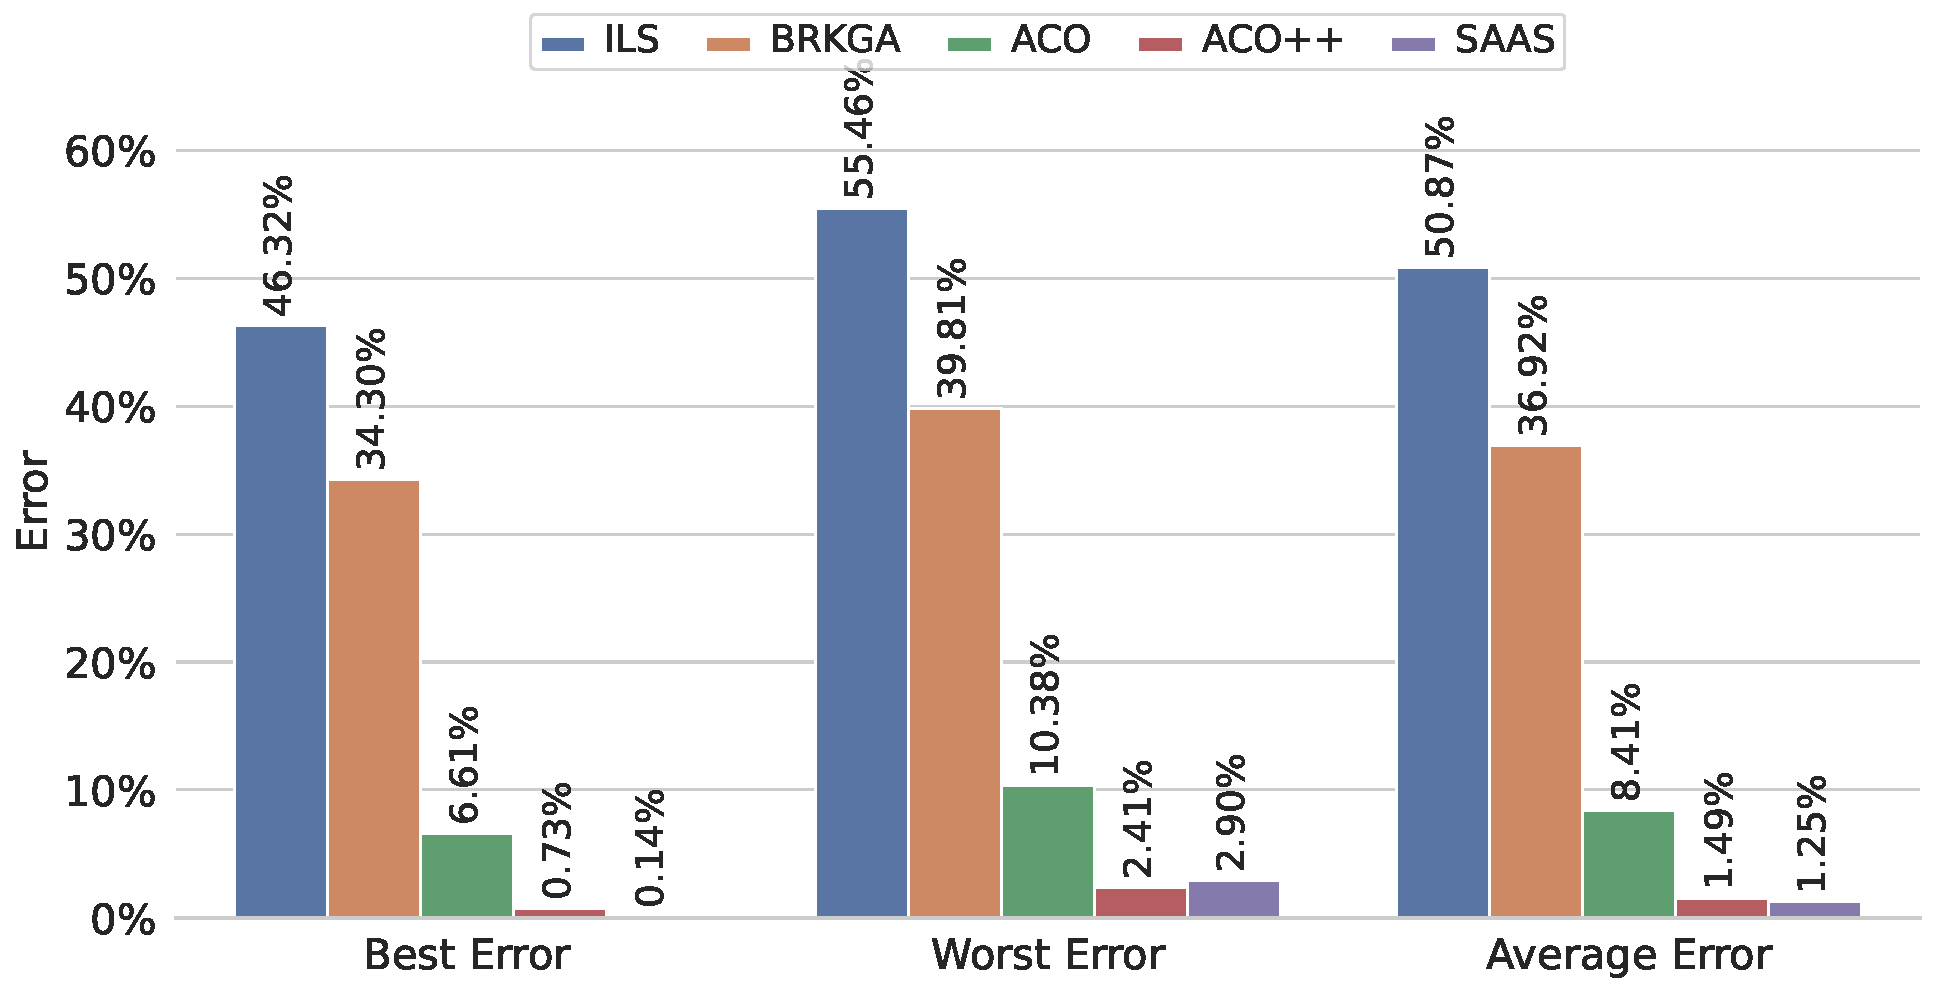
\includegraphics[width=\linewidth]{Figures/error_rate.pdf}
  \caption[Kết quả thực nghiệm so sánh độ chênh lệch của lời giải của các thuật toán.]{Biểu đồ cột thể hiện độ chênh lệch của lời giải của mỗi thuật toán so với lời giải tốt nhất tìm được. Biểu đồ thể hiện 3 cách tính độ chênh lệch: độ chênh lệch tốt nhất, độ chênh lệch tệ nhất, và độ chênh lệch trung bình.}
  \label{fig:errorRate}
\end{figure}
% \subsection{Thông tin cấu trúc của lời giải tốt nhất được tìm thấy}
% \label{sec:soltruc}
% \begin{table}
%     \begin{center}   
%         \begin{tabular}{llrrrrrrrr}
%             \toprule
%             % \multirow{2}{3em}{\texttt{XXX}} & \multirow{2}{2em}{\texttt{YY}} & \multicolumn{3}{c}{ACO++} &&  \multicolumn{3}{c}{SAAS}\\
%             \multicolumn{2}{c}{trường hợp group}& \multicolumn{3}{c}{ACO++} &&  \multicolumn{3}{c}{SAAS}\\
%             \cline{3-5}\cline{7-9}
%             \texttt{XXX} & \texttt{YY} &\multicolumn{1}{c}{$\mathcal{D}$} & \%T & \%W &&\multicolumn{1}{c}{$\mathcal{D}$} & \%T & \%W \\
%             \midrule
%             \multirow{4}{3em}{eil51}    & 01 &              10.469 &           98.994 &  \textbf{79.551} &   &     \textbf{10.447} &  \textbf{99.123} &           79.533 \\
%                                         & 03 &               8.646 &           99.592 &  \textbf{85.066} &   &      \textbf{8.636} &  \textbf{99.668} &           84.939 \\
%                                         & 05 &      \textbf{8.517} &  \textbf{99.759} &           85.412 &   &                8.53 &           99.731 &  \textbf{85.514} \\
%                                         & 10 &      \textbf{8.204} &           99.865 &  \textbf{86.544} &   &               8.243 &  \textbf{99.913} &            86.52 \\
%             \midrule
%             \multirow{4}{3em}{pr107}    & 01 &             682.053 &           99.686 &  \textbf{81.697} &   &    \textbf{663.738} &   \textbf{99.77} &  \textbf{81.697} \\
%                                         & 03 &             477.944 &  \textbf{99.931} &           83.823 &   &    \textbf{476.552} &           99.894 &  \textbf{84.443} \\
%                                         & 05 &             447.241 &           99.939 &           84.173 &   &    \textbf{437.632} &  \textbf{99.943} &  \textbf{85.575} \\
%                                         & 10 &             417.133 &           99.881 &           84.728 &   &    \textbf{414.535} &  \textbf{99.949} &  \textbf{85.576} \\
%             \midrule
%             \multirow{4}{3em}{a280}     & 01 &      \textbf{14.11} &           99.815 &  \textbf{84.743} &   &              14.155 &  \textbf{99.838} &           84.651 \\
%                                         & 03 &     \textbf{10.405} &           99.763 &  \textbf{85.825} &   &              10.462 &  \textbf{99.937} &           85.735 \\
%                                         & 05 &      \textbf{9.651} &           99.917 &            86.33 &   &               9.736 &  \textbf{99.935} &  \textbf{86.493} \\
%                                         & 10 &      \textbf{9.216} &           99.961 &           86.126 &   &               9.419 &  \textbf{99.964} &    \textbf{86.2} \\
%             \midrule
%             \multirow{4}{3em}{dsj1000}  & 01 &  \textbf{37309.633} &           72.359 &  \textbf{86.171} &   &           41557.939 &  \textbf{74.142} &           85.822 \\
%                                         & 03 &  \textbf{18960.953} &           99.937 &  \textbf{89.691} &   &           19286.319 &  \textbf{99.964} &           89.598 \\
%                                         & 05 &           18034.123 &  \textbf{99.959} &           90.059 &   &  \textbf{17868.094} &           99.795 &  \textbf{90.364} \\
%                                         & 10 &  \textbf{17694.494} &  \textbf{99.692} &  \textbf{90.497} &   &           17737.117 &           99.664 &            90.44 \\
%             \midrule
%             \multicolumn{2}{c}{Total}  & 9 & 4 & 9 && 7 & 12 & 8  \\
%             \bottomrule
%         \end{tabular}
%         \caption[Thông tin cấu trúc của lời giải tốt nhất được tìm thấy của ACO++ và SAAS]{
%         \label{tab:soltruc}Thông tin cấu trúc của lời giải tốt nhất được tìm thấy. Giá trị in đậm thể hiện yếu tố đó của thuật toán hiệu quả hơn so với thuật toán còn lại.}
%     \end{center}
% \end{table}